%%This is a very basic article template.
%%There is just one section and two subsections.
\documentclass{article}

\usepackage{amsmath}
\usepackage{caption}
\usepackage{placeins}
\usepackage{graphicx}
\usepackage{subcaption}
\usepackage{tikz}
%\usepackage[active,tightpage]{preview}
\usepackage{natbib}
\bibpunct{(}{)}{,}{a}{}{;} 
\usepackage{url}
\usepackage{nth}
\usepackage{authblk}
% for the d in integrals
\newcommand{\dd}{\; \mathrm{d}}
\newcommand{\tc}{\quad\quad\text{,}}
\newcommand{\tp}{\quad\quad\text{.}}
\defcitealias{HMD}{HMD}

\begin{document}


\title{Life lost, lifesaving, and causes of death.}

\author[1]{Tim Riffe}
\author[2]{A{\"i}da Sole Auro}
\affil[1]{Department of Demography, University of California, Berkeley}
\affil[2]{Institut National d'{\'e}tudes d{\'e}mographiques}
% A{\"i}da Sole Auro
\maketitle

\begin{abstract}
The lives and potential years of life lost due to death are presented as metric
for describing the population impacts of death and for comparing causes of
death. Lost lives and years of life may be classified by the ages in which
deaths occurred, by the ages to which deaths would be postponed were they saved, by the
ages in which the lost years would have been lived, or by the distribution of
lost remaining lifespans. These temporal perspectives define the
potential impacts of death and causes of death on population size and structure,
and on the distribution of lifespans within populations. 
\end{abstract}

\section*{Temporal relationships}
%To begin, assume a closed population and ignore what determines the size of
%successive birth cohorts, $B(t)$, which we usually call the birth flow. If
%$B(t)$ is a given, then the only other factor that determines population size
%and age structure is the length of the lives of its members. For simplicity,
%assume that the age pattern to mortality is fixed (this isn't necessary, but it
% simplifies notation). The population of age $a$ in year $t$, $P(a,t)$, is a function of the survival of the birth cohort born in year $t-a$. Since we're
%fixing mortality, survival from age 0 to $a$ is $l(a)$ for any given cohort, so
%$P(a,t) = B(t-a)l(a)$.

Population stock in a given year, $t$, can be structured by birth
cohorts or age, the way we typically make population pyramids. If an entire
lifespan is denoted by the random variable, $X$, then the remaining lifespan,
$y$, of a still-alive person aged $a$, $y = X - a$. 
\begin{figure}[h]
\centering
	\caption{A lifeline, where chronological age (years lived) is indexed by $a$
	and thanatological age (years left) is indexed by $y$.}
	\label{fig:line}
	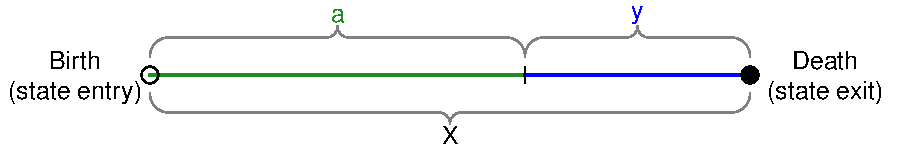
\includegraphics[scale=.8]{Figures/LifeLine.pdf}	
\end{figure}
Figure~\ref{fig:line} gives a schematic representation of this simple
relationshp, which generalizes to other durations or state transitions. For a
cohort, the distribution of $X$ is given by $f(X)$, which is equal to the familar lifetable
$d(a)$ for $a = X$, when specified with a radix of 1. The distribution of
\textit{remaining} lifetimes for those having survived to age $a$, $f(y|a)$ is
given by:\footnote{Equation \eqref{eq:fya} is easily modifiable to account for
mortality schedules that change over time.}
\begin{equation}
\label{eq:fya}
f(y|a) = \mu(a+y) \frac{l(a+y)}{l(a)} \tc
\end{equation}
where $\mu(a)$ is the force of mortality at exact age $a$, and $l(a)$ is
the value of the survival function at exact age $a$, the probability of
surviving from birth to age $a$. Figure~\ref{fig:fya} shows selected
cross-sections of the $f(y|a)$ surface calculated from the 2010 US male period lifetable (HMD). 
\begin{figure}[h]
\centering
	\caption{US males, 2010, $f(y|a)$ for selected ages.*}
	\label{fig:fya}
	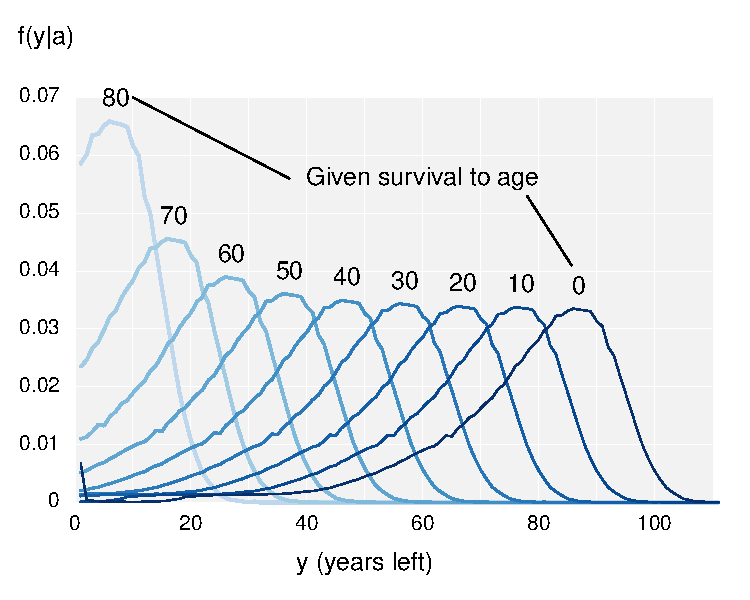
\includegraphics[scale=.8]{Figures/fya.pdf}	
	\caption*{*Data from \citetalias{HMD}. Note that $f(y|0) = d(a) = f(X)$.}
\end{figure}
$f(y|a)$ can be used to calculate the population having survived to age $a$ and
with $y$ remaining years of life as $P(a,y) = P(a)f(y|a)$, where the total
population with $y$ remaining years of life, $P(y)$, is simply $\int
_{a=0}^\infty P(a,y) \dd a$, a single death cohort with members from many birth
cohorts. This decomposition sorts the lifeline segments of a living population
by the part yet-unlived (years left) rather than by the part lived. The lived
part we call ``age'' and the unlived part has no common name. Since age is a
placemarker on the lifeline, both $a$ and $y$ could be called ``age'', and we
can specify them as \textit{chronological} and \textit{thanatological} age,
respectively.\footnote{Thanatos was the Greek god of death, which marks the end of the lifeline to which $y$ relates. By this token, one could just call chronological age \textit{aphrodesian} age, but this would probably confuse things.}

The indices $a$ and $y$ differentiate between the past and future
parts of a lifeline, respectively, and by extension of populations when
so structured.
In comparing $P(a)$ with $P(y)$, as in \citet{brouard1986structure}, we still
refer to the living (lived or to-be-lived) part of a population.
Is it so clear that the dead are no longer part of the population? If a life is
completely saved, this life stays in the living population and is not counted
as a death, but we (in common thinking) often imagine saved lives as a transient
state classification.
Perhaps this is not correct for demographers: amongst the living there
are no saved lives but only lived lives. Still we can quantify
hypothetically saveable life, and for this we must look to deaths.
It is nice (and often realistic) to think that many of the lives taken by death are (or will one day be) saveable, but little demography has been done of the lives that could be saved. If a saved life joins back into (so to speak) the homogeneous pool of alive people (the simplest way
to proceed), one may ask much more than how many lives can be saved, $D^s(a)$
(saveable lives, the number of real or would-be deaths at age $a$)
\begin{equation}
D^s(a) = \mu(a)P(a) \quad \quad \text{,}
\end{equation}
but also how many years would the people saved at age $a$ live,
$W^s(a)$\footnote{A mnemonic for $W$ could be \textit{won} years.}? The simplest
calculation is to multiply the number of gained survivors by remaining life expectancy, $e(a)$:
\begin{align}
\label{eq:savedea}
W^s(a) = D^s(a)e(a) &= P(a)\mu(a)\frac{1}{l(a)}\int_{y=0}^\infty l(a+y) \dd y
%\notag\\
         %&= \mu(a)\int_{y=0}^\infty B(t-a)l(a+y) \dd y 
\end{align}
$D^s(a)e(a)$ classifies potentially saved person-years by the
ages in which they were saved. Figure~\ref{fig:Day} (left) shows US 2010 period
deaths (all the lives that could be saved) by age and sex (males on the left,
females on the right). Over 1.23 million deaths were recorded for males
and females each in 2010 in the US. Deaths have been decomposed into discrete
categories of remaining years of life using equation~\eqref{eq:fya}, under the assumption that saved lives are subject to the same mortality schedule as the rest of the population, and under the supposition that all 2010 deaths get saved (just once). The results of this decompositon are represented by color bands in
Figure~\ref{fig:Day}. Figure~\ref{fig:Dya} (right) displays the same
information after flipping the y axis and color gradient from
Figure~\ref{fig:Day}. Now the remaining lifespans (years left) of
hypothetically saved lives are the primary y axis, while ages (years lived)
are displayed with color. Figure~\ref{fig:Dya} communicates that most saveable
lives would live short remaining lifespans once saved and granted the same lifetable
mortality. This is so because most saveable lives are already in high
chronological ages. In general, the only saveable lives that might live very
long remaining lifespans are the few deaths that occur in young ages.

\begin{figure}
\centering
\caption{US, 2010 potentially saveable lives (Deaths)*}
\label{fig:1}
\begin{subfigure}[b]{.48\linewidth}
\centering
	\caption{Classified by age (years lived) and sex, and decomposed
by hypothetical remaining years of life (years left).}
	\label{fig:Day}
	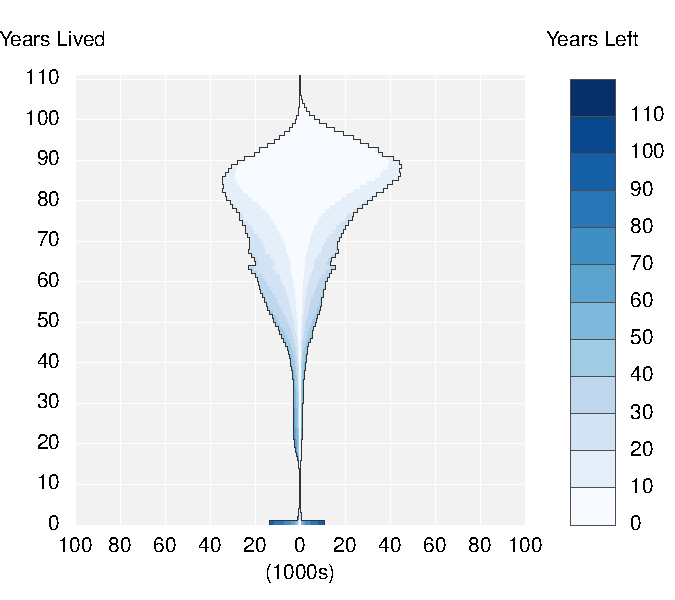
\includegraphics[scale=.55]{Figures/Deathsxy10.pdf}	
\end{subfigure}
~
\begin{subfigure}[b]{.48\linewidth}
\centering
    \caption{Classified by hypothetical remaining years of life
(years left) and sex, and decomposed by age (years lived).}
	\label{fig:Dya}
    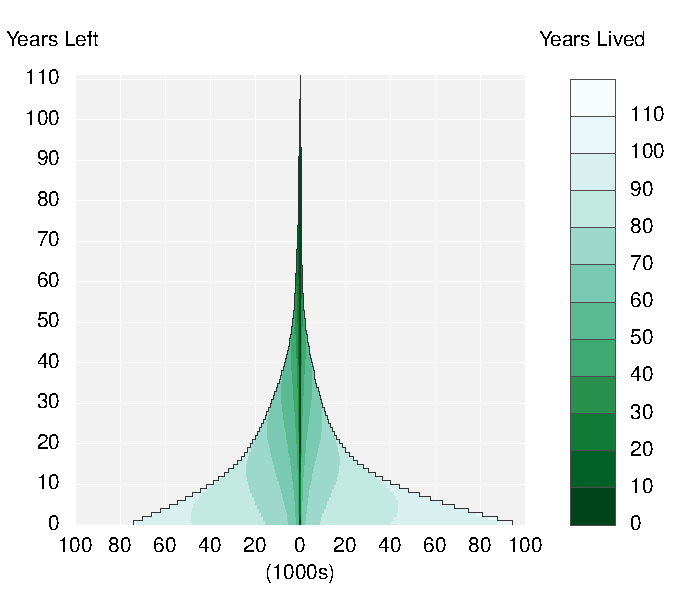
\includegraphics[scale=.55]{Figures/Deathsyx10.pdf}
\end{subfigure}
\caption*{*Data from \citetalias{HMD}}
\end{figure}

\begin{figure}
\centering
\caption{US, 2010 person years of life potentially won*}
\label{fig:2}
\begin{subfigure}[b]{.48\linewidth}
\centering
	\caption{Classified by age at saving and sex, $W^s(a)$, and decomposed by
	future ages to be lived.}
	\label{fig:SavedGained}
	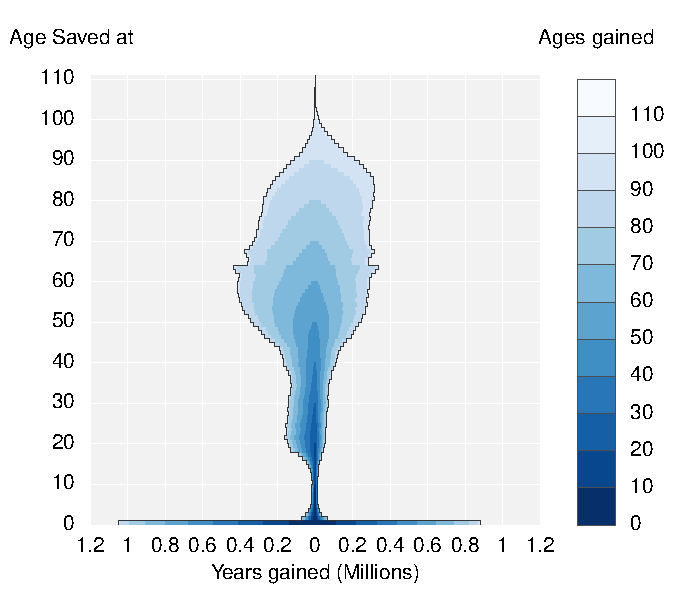
\includegraphics[scale=.55]{Figures/YearsSavedGainedxx10.pdf}	
\end{subfigure}
~
\begin{subfigure}[b]{.48\linewidth}
\centering
    \caption{Classified by future ages to be lived and sex, and decomposed
    by age at saving.}
	\label{fig:LostLived}
    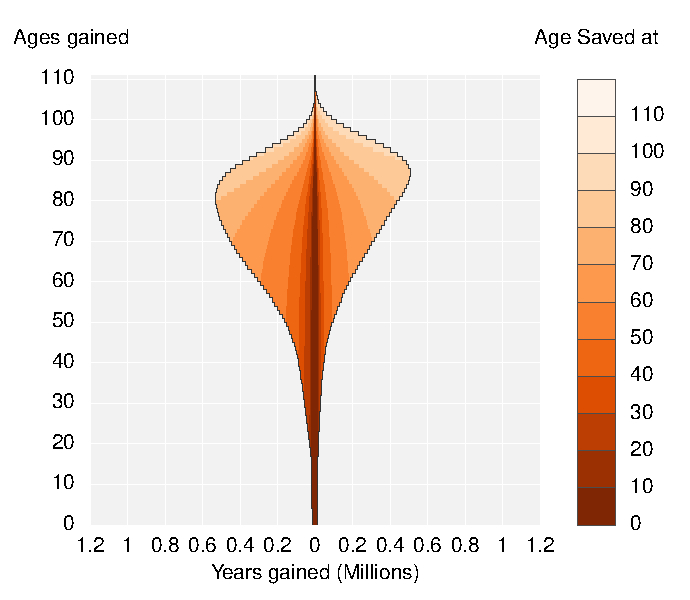
\includegraphics[scale=.55]{Figures/YearsLostLivedyx10.pdf}
\end{subfigure}
\caption*{*Data from \citetalias{HMD}. (Note different x scale from
Figure~\ref{fig:1}).}
\end{figure}
Figure~\ref{fig:SavedGained} shows the results of applying
equation~\eqref{eq:savedea} to the same US data, which is essentially a
reweighting of Figure~\ref{fig:Day} by remaining life expectancy. Color bands
are assigned by decomposing the total life to be lived into the ages through
which it will be lived. For example, if we save all 11700 of the 50-year-old
males that died in 2010, they would live a total of 349000 combined years (under
constant and homogenous mortality), spread out over ages 50 and higher according
to $f(50+y|50)$. In Figure~\ref{fig:SavedGained} we decompose these gained
years of life according to equation\eqref{eq:savedy} (using $f(a+y|a)$) and
highlight this decomposition with color, while in Figure~\ref{fig:LostLived}, \textit{gained} ages become the primary y axis,
while color bands represent the ages in which populations in each age group were
saved. Figure~\ref{fig:LostLived} represents the cumulative contribution to the
population pyramid that would result from saving all lives in 2010 and then
surviving them forward according to 2010 mortality conditions.

One may also wish to know the distribution of remaining lifespans of saved
lives, which is quite different from \eqref{eq:savedea}:\footnote{Under constant mortality, but
not-necessarily constant fertility, this simplifies to $D^s(a)f(y|a) =
B(t-a)\mu(a)\mu(a+y)l(a+y)$}
\begin{equation}
\label{eq:savedy}
D^s(a)f(y|a) = P(a)\mu(a)\mu(a+y) \frac{l(a+y)}{l(a)} \tc
\end{equation}
or indeed the time-to-death distribution of the total years of life
gained:\footnote{not yet included in figures, coming soon.}
\begin{equation}
\label{eq:gainedy}
W^s(y) = \int_{a=0}^\infty D^s(a)\frac{l(a+y)}{l(a)} \dd a \tc
\end{equation}
or indeed the ages in which the gained years of life would be lived,
$W^s(a+y|a)$:
\begin{equation}
\label{eq:gaineday}
W^s(a+y|a) = D^s(a)\frac{l(a+y)}{l(a)} \tc
\end{equation}
A bit more description to come here.

\section{Extention to causes of death.}
These basic relationships carry over when deaths and survival are adjusted to
account for the hypothetical elimination of particular causes (in the case of
exclusivity). In this case $D^s$ is the sum of $c$ causes, and to speak of
eliminating cause $c$ from the lifetable is to speak of saving $D^{sc}$ lives and then
subject them to the mortality conditions of all causes except $c$.
This is problematic in that causes are not exclusive, and also in that we do not
truly eliminate causes entirely over all ages, but it serves as a good basis for comparing the relative
impacts of different causes on a given population structure. Similarity between
temporal patterns of saveable cause-specific remaining lifespans might also
serve as an ad hoc basis for judging how much particular causes actually compete
as risks, wherein true ersatz causes will have similar distributions (and so may
be grouped).

Let us then define the force of mortality, $\mu(a) = \sum _{c=1}^n \mu^c(a)$,
as the sum of $n$ categorically separable causes. The people that will die from
cause $c$ are:
\begin{align}
D^c &= \int_0^\infty D^c(a) \dd a \\
&= \int_0^\infty \mu^c(a)P(a) \dd a \tc\\
\intertext{and to hypothetically save all these people is to remove cause $c$
from mortality, retaining $D^c$ lives in the population. It makes sense to
calculate the distribution of remaining lifespans of the $D^c$ people that would
have died of this cause using $l(a)$ removed of the cause in question, so we define
$l^{-c}(a)$:}
l^{-c}(a) &= e^{-\int _0^a \mu(a)-\mu^c(a) \dd a} \tc\\
\intertext{which is hopefully more legible to render as:}
l^{-c}(a) &= e^{-\int _0^a \mu^{-c}(a) \dd a} \tp\\
\intertext{Continue with the same notational concept of ${ }^{-c}$ to define
remaining life expectancy assuming survival to age $a$ and no more death from
cause $c$ after age $a$, $e^{-c}(a)$:}
e^{-c}(a) &= \frac{1}{l^{-c}(a)}\int _y^\infty l^{-c}(a+y) \dd y \tp
\end{align}
and so on, repeating equations \eqref{eq:savedea} and \eqref{eq:savedy} for the
case of cause-specific saveable lives and their cause-deleted remaining
lifespans.

Figures to be repeated for a sample cause of death, probably external causes.

\section{Observed patterns}


\bibliographystyle{plainnat}
  \bibliography{references}  
\end{document}
